%%%%%%%%%%%%%%%%%%%%%%%%%%%%%%%%%%%%%%%%%
% Original author:
% Linux and Unix Users Group at Virginia Tech Wiki
% (https://vtluug.org/wiki/Example_LaTeX_chem_lab_report)
% Modified by: Hector F. Jimenez S, for the Digital Electronics Laboratory.
% License:
% CC BY-NC-SA 3.0 
%%%%%%%%%%%%%%%%%%%%%%%%%%%%%%%%%%%%%%%%%
%----------------------------------------
%	PACKAGES AND DOCUMENT CONFIGURATIONS
%---------------------------------------
\documentclass[paper=a4, fontsize=12pt]{article} 		% A4 paper and 11pt font size
\usepackage[T1]{fontenc} 								% Use 8-bit encoding that has 256 glyphs
%\usepackage{fourier}		 							% Use the Adobe Utopia font for the document 
\usepackage[spanish,english]{babel}						% Spanish Language, templates uses some sections in english.
\selectlanguage{spanish}								% main language.
\usepackage{subfig}
\usepackage{multirow}
\PassOptionsToPackage{spanish}{babel}
\renewcommand{\figurename}{Figura}						% Force rename of figure.
\renewcommand{\figurename}{Fig.}
\usepackage[figurename=Fig.]{caption}
\usepackage[utf8]{inputenc}								% tildes for spanish language.
\usepackage{amsmath,amsfonts,amsthm} 					% Math packages.
\usepackage{minted}										% For syntax highlighting.
	    \renewcommand\listingscaption{Código}			%rename the source code minted !
\usepackage{float}										% Image will be in the same place as you want.!!! x-/
\usepackage{sectsty} 									% Allows customizing section commands
\allsectionsfont{\centering \normalfont\scshape}	   	% Make all sections centered, the default font and small caps
\usepackage{hyperref}
\hypersetup{											%Setups the false color and borders.
    colorlinks=false,
    pdfborder={0 0 0},
}
\newcommand\fnurl[2]{%									% set a simple and quick footnote command and include url.
\href{#2}{#1}\footnote{\url{#2}}%	
}
\usepackage{graphicx}									% Import easyly images.
\graphicspath{ {./images/} }							% Where to look for the images.
\DeclareGraphicsExtensions{.pdf,.png,.jpg}				% Graphics Extension to be used
\usepackage[notes,backend=biber]{biblatex-chicago}		% Bibliography and references.
\bibliography{biblio}									% bibliography filename.
\usepackage{fancyhdr} 									% Custom headers and footers
\pagestyle{fancyplain} 									% Makes all pages in the document conform to the custom headers and footers
\fancyhead{} 											% No page header
\fancyfoot[L]{} 										% Empty left footer
\fancyfoot[C]{} 										% Empty center footer
\fancyfoot[R]{\thepage} 								% Page numbering for right footer
\renewcommand{\headrulewidth}{0pt} 						% Remove header underlines
\renewcommand{\footrulewidth}{0pt} 						% Remove footer underlines
\setlength{\headheight}{13.6pt} 					    % Customize the height of the header
\numberwithin{equation}{section}						% Number equations within sections (i.e. 1.1, 1.2, 2.1, 2.2 instead of 1, 2, 3, 4)
%\numberwithin{figure}{section} 						% Number figures within sections (i.e. 1.1, 1.2, 2.1, 2.2 instead of 1, 2)
\numberwithin{table}{section} 							% Number tables within sections (i.e. 1.1, 1.2, 2.1, 2.2 instead of 1, 2, 3, 4)
\setlength\parindent{0pt} 								% Removes all indentation from paragraphs
\newcommand{\horrule}[1]{\rule{\linewidth}{#1}} 		% Create horizontal rule command with 1 argument of height
\usepackage{listings}% http://ctan.org/pkg/listings
\usepackage{multicol}
\usepackage{caption}
\usepackage{subfig}
\renewcommand{\lstlistingname}{Código}	
\title{Sistemas Operativos I\\ 
\horrule{0.5pt} \\[0.4cm] 								% Thin top horizontal rule	Title rule
\textit{Taller 9: Caso de estudio del sistema operativo Chrome OS}
\horrule{1pt} \\[0.5cm] 			
} 			

\author{												
Héctor F. \textsc{Jiménez Saldarriaga.}\\				% Authors begin.
\texttt{hfjimenez@utp.edu.co} \\						
\texttt{PGP KEY ID: 0xB05AD7B8}
} 
% End of  Author name
\date{}    						                       % Date for the report, this will hide the \today.

\begin{document}
\maketitle                      			           % Insert the title, author and date
\begin{center}
\begin{tabular}{l r}								   % two column to
Fecha de Entrega: & Marzo, 2018 \\				   % Ramiro's Details.
Profesor: & Cesar Manuel Castillo Rodriguez
\end{tabular}
\end{center}
%%%%%%%%%%%	
% Let's start the document.
%%%%%%%%%%%	
\section{Objetivos}
\begin{itemize}
	\item Evolución
	\item Realizar el proceso de instalación del sistema operativo	
    \item Identificar el manejo de Archivos, Shell
    \item Estructura del Sistema Operativo
    \item Clasificación del Sistema Operativo
\end{itemize}
\section{Evolución de Chrome OS} 
%Formato imagen unica
\begin{center}
\begin{figure}[H]
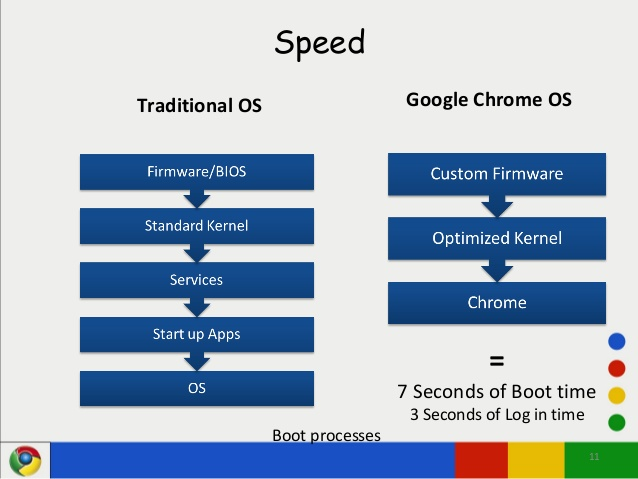
\includegraphics[scale=0.6]{imgs/design.jpg}
\caption{Arquitectura y diseño de Chrome OS}
\label{fig:dis2}
\end{figure}
\end{center}

Google Chrome OS es un proyecto llevado a cabo por la compañía Google para desarrollar un sistema operativo basado en web. A través de su blog oficial, Google anunció el 7 de julio de 2009 Google Chrome OS, un sistema realizado con base en código abierto (Núcleo Linux) y orientado inicialmente para miniportátiles, estando disponible en junio de 2011.Funciona sobre microprocesadores con tecnología x86 o ARM.


El 7 de julio de 2009, Google anuncia uno de sus más grandes proyectos, su propio sistema operativo, el cual es nombrado «Google Chrome OS» (o simplemente abreviadoChrome OS), justo 9 meses después de haber lanzado su navegador Google Chrome.

Las primeras características que destaca Google es, que su sistema operativo es un proyecto de código abierto y sin costo alguno. Al igual que el navegador Google Chrome que cuenta con el proyecto Chromium como el proyecto abierto para su desarrollo, Google Chrome OS cuenta con Chromium OS como proyecto de código abierto para su desarrollo. Google también destaca que su interfaz de usuario es simple, rápida, y segura, debido a que su principal herramienta de uso es el navegador Google Chrome. El sistema operativo está diseñado de tal forma que el usuario pueda conectarse a Internet en cuestión de segundos.
\subsection{UX Interfaz de usuario}
Al momento de realizar la instalacion de este sistema operativo todo parece un poco confuso pues lo unico con lo que contamos es un navegador web y tal y sus principales características de la interfaz de usuario son:
\begin{itemize}
\item \textbf{Paneles}: Los paneles son pequeñas ventanas inferiores que se utilizan para diferentes tareas, tales como la descarga de archivos, navegador de archivos, mensajería instantánea en Gtalk, tomar notas, o notificadores de eventos como Google Calendar, Gmail, y actualizaciones del sistema. Los paneles también permiten ser minimizados para ocultarse, y también se pueden utilizar mientras se navega en diferentes sitios al permanecer estáticos.
\item \textbf{Indicadores}: Los indicadores se encuentran en la parte superior derecha, e indican procesos como la hora, batería, conexión y selector Wi-fi, y conexión 3G.
\item \textbf{Pestañas}: Las pestañas son lo más utilizado en el sistema, se utilizan para abrir las aplicaciones y sitios, y permiten abrir opciones del sistema. Las pestañas también se pueden "fijar" y disminuir su tamaño para quedar ancladas en la parte superior izquierda.
\item \textbf{Lanzadores}: Los lanzadores aparecen en la página principal, y son iconos grandes que se utilizan para abrir aplicaciones web, también ver los sitios más visitados, y ver los marcadores en una barra superior.
\end{itemize}
\subsection{Aplicaciones Web }
Chrome OS no utiliza el típico sistema de aplicaciones, las aplicaciones se utilizan dentro del navegador web Google Chrome, y pueden ser utilizadas en línea o ser instaladas para poder utilizarse sin la necesidad de una conexión a Internet. El principal medio para obtener estas aplicaciones web es la tienda en línea Chrome Web Store, la cual permite adquirir aplicaciones, extensiones y temas para el navegador Google Chrome en un solo lugar. La tienda también permite comprar aplicaciones, y que los desarrolladores publiquen sus aplicaciones basadas en lenguaje web actual.
\subsection{Seguridad }
También contará con una arquitectura de seguridad actualizada. Google enfatiza el hecho de que sus Chromebooks no sufrirán de virus o programas maliciosos. Debido a que muchos sistemas operativos actuales fueron diseñados en épocas en las que internet no era predominante, Chrome se diseña teniendo muy en cuenta esto, por ende eliminando riesgos de seguridad comunes arraigados.
Los puntos más importantes con respecto a la seguridad de Chrome OS son:
\begin{itemize}
\item Actualizaciones automáticas: Las aplicaciones webs instaladas, extensiones, temas, el navegador, y el sistema operativo se mantendrá al día con actualizaciones automáticas.
\item     Aislamiento de procesos: Aislar procesos que puedan comprometer la seguridad del sistema, tales como Flash Player, extensiones o aplicaciones instaladas.
\item     Verificación de arranque: Monitorea si el sistema ha sido manipulado por entes externos antes de que el sistema parta, y vuelve a una versión de respaldo si esto ha sucedido.
\item     Cifrado de datos: Todos los datos descargados en el disco son cifrados.
\item     Modo visita: Parecido a la «cuenta de invitado» presente en sistemas operativos Windows, GNU/Linux, y Mac OS X. En este modo el usuario puede pasar la máquina a conocidos para que utilicen una cuenta de visita sin que sus datos se vean comprometidos.
\end{itemize}
\subsection{Chromebooks}
El 11 de mayo de 2011, en el evento Google I/O son presentados dos Chromebooks potenciados con Chrome OS, fabricados porSamsung y Acer. Ambos Chromebooks cuentan con discos SSD, sin unidad óptica, tapete multitáctil, pantallas de 12,1 y 11,6 pulgadas, conexión Wi-Fi o 3G, y con baterías de larga duración de hasta 8,5 horas continuas. El 15 de junio de 2011 los Chromebooks se lanzaron a la venta para el público, con precios desde los $349 hasta los $499 USD.Actualmente se consiguen apartir de 150 USD.Google trabaja con numerosas empresas para diseñar y construir dispositivos que soporten Chrome OS, chromium os. Entre la lista de empresas destacan Intel, Acer, Samsung,Adobe, ASUS, Freescale, Hewlett-Packard, Lenovo, Qualcomm, Texas Instruments, Canonical, Dell y Toshiba.

\begin{center}
\begin{figure}[H]
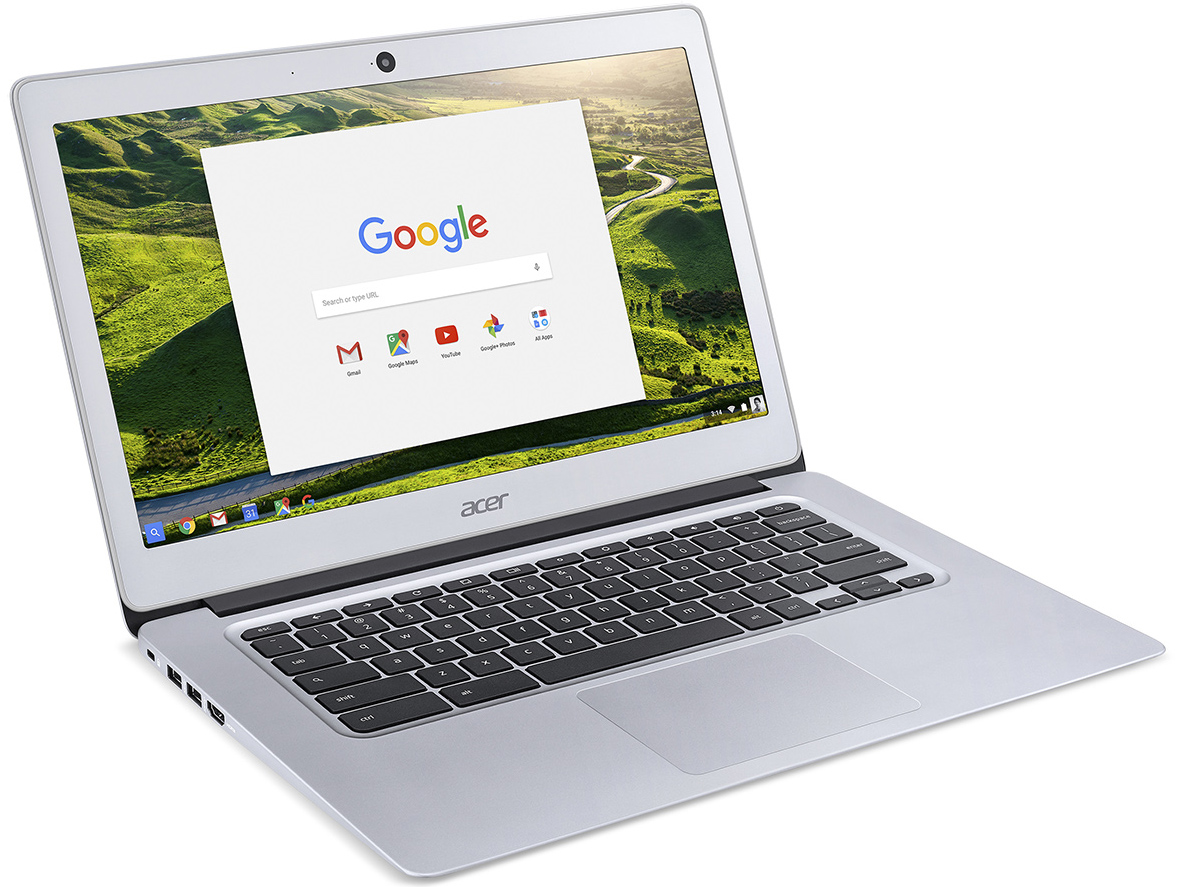
\includegraphics[scale=0.4]{imgs/qwe_download.jpeg}
\caption{Chrome OS, Una de las primeras maquinas de ACER con sistema operativo precargado}
\label{fig:dis2}
\end{figure}
\end{center}

\section{Proceso de instalación Chrome OS}
El proceso para realizar la instalación de este sistema operativo es obtener una imagen virtualizada de una empresa que se dedica a dar soporte comercial Chrome OS, ellos liberan versiones para realizar pruebas en maquinas virtuales, para este caso se realizaron multiples intentos fallidos con Virtualbox pero finalmente me percate que la imagen era para WMWare Player o Workstation.
\begin{figure}[H]
 	\centering
   	\subfloat[Bienvenida Instalador Chrome OS,]{\label{fig:bienvenida}{
   		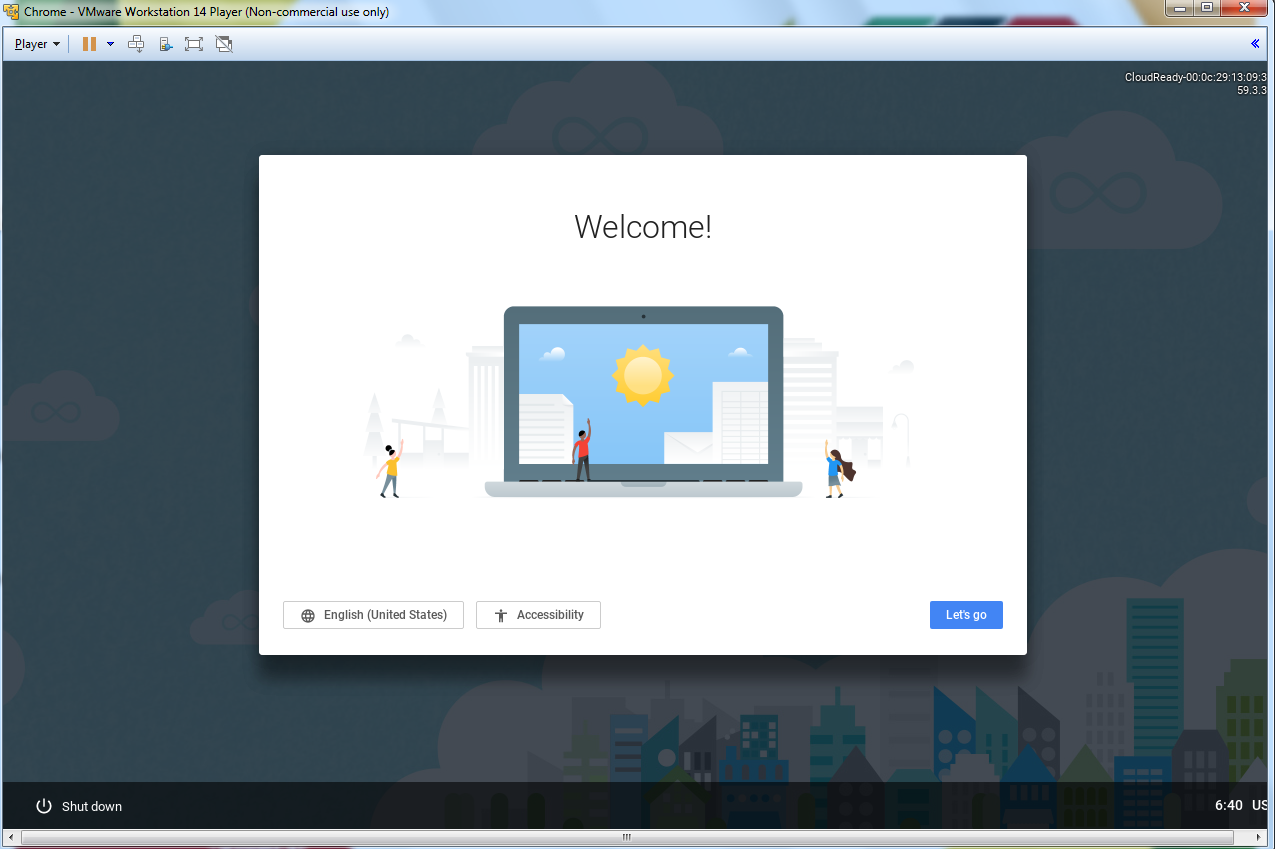
\includegraphics[width=0.68\textwidth]{imgs/2.png}
   		}}
	\subfloat[S]{\label{fig:formateada}{
   		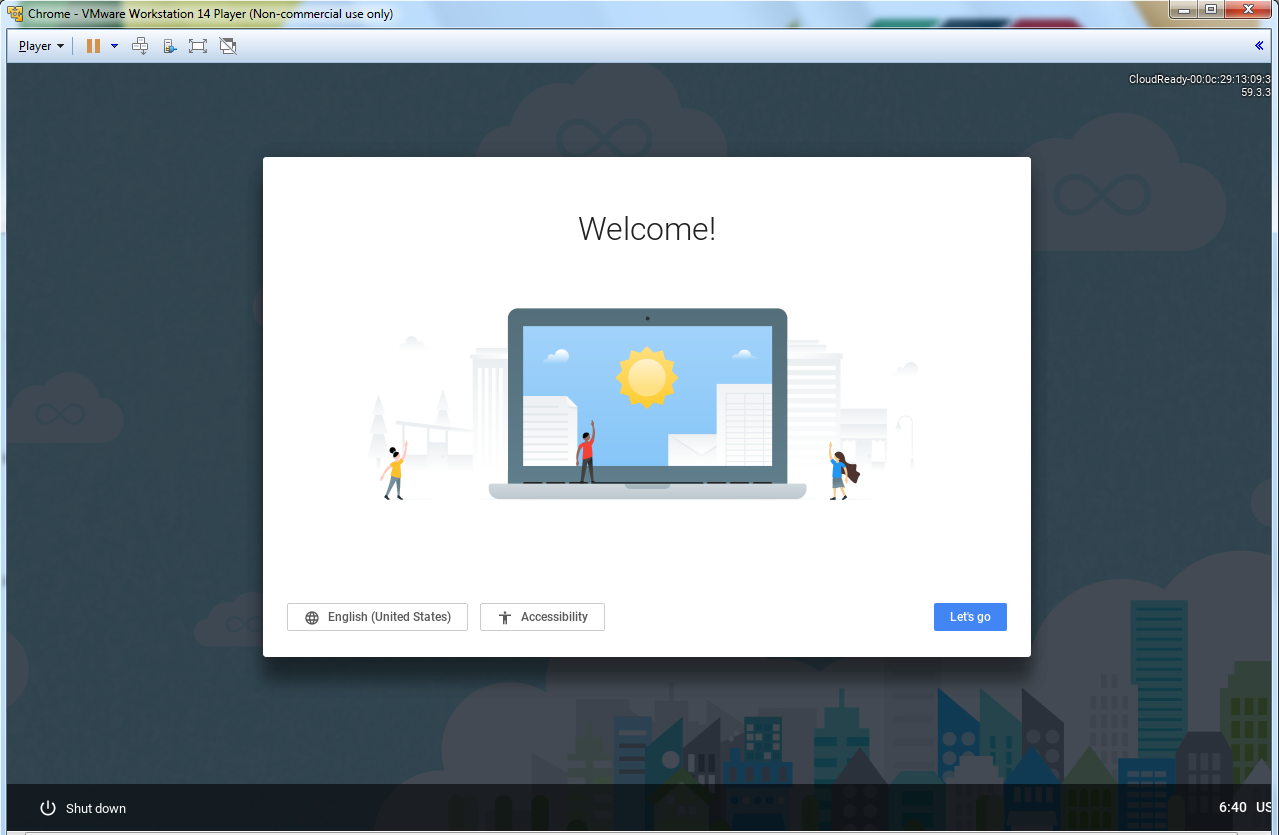
\includegraphics[width=0.68\textwidth]{imgs/3.png}
        }}
       \hfill
	\subfloat[Seleccion de Idioma y teclado.]{\label{fig:disco}{
   		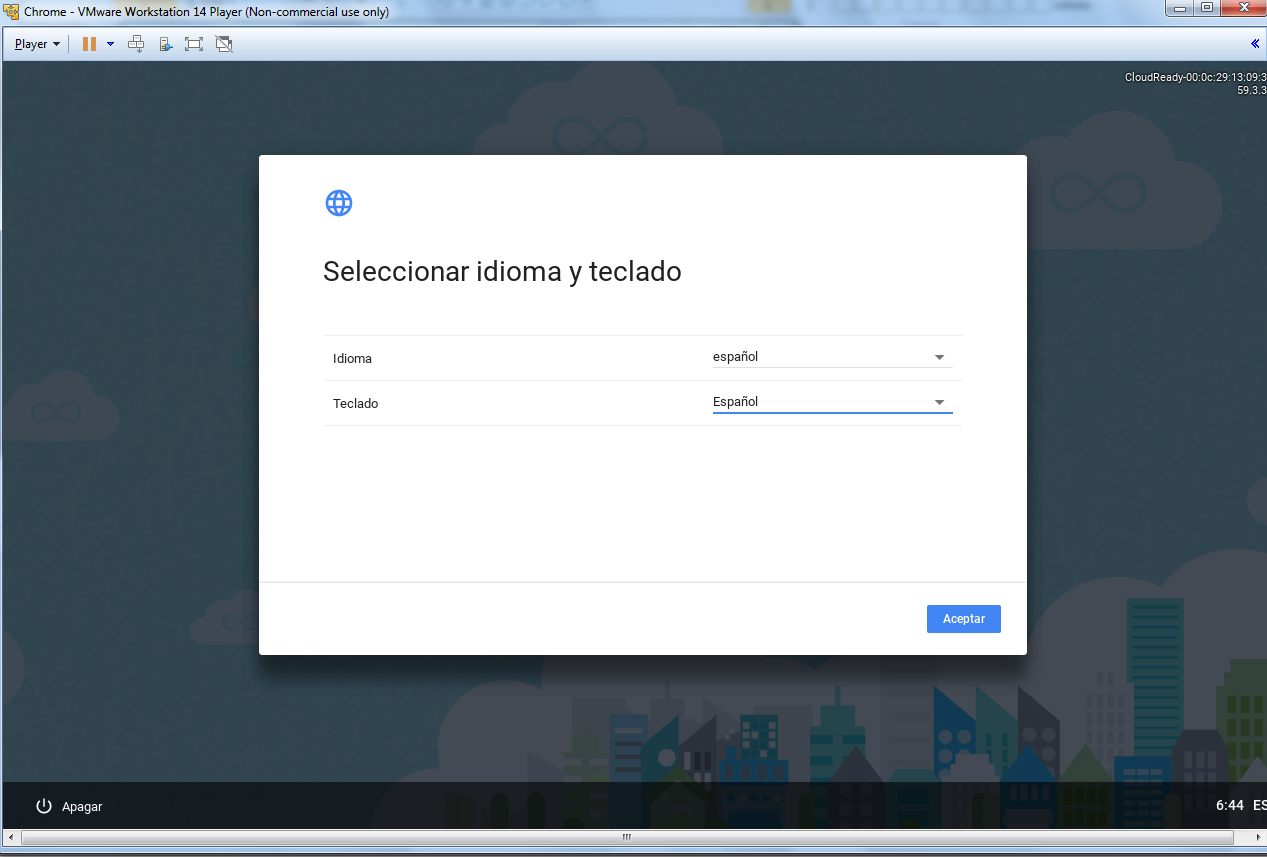
\includegraphics[width=0.68\textwidth]{imgs/4.png}
        }}
	\subfloat[Inicio de Session para iniciar usando el chromebook]{\label{fig:ufs}{
   		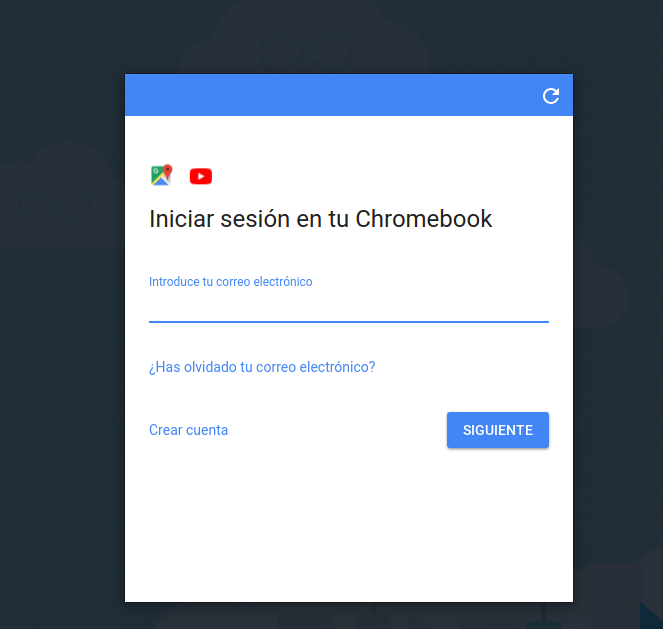
\includegraphics[width=0.68\textwidth]{imgs/5.png}
        }}
        \hfill
	\subfloat[Personalizacion Imagen de usuario]{\label{fig:confirmar}{
   		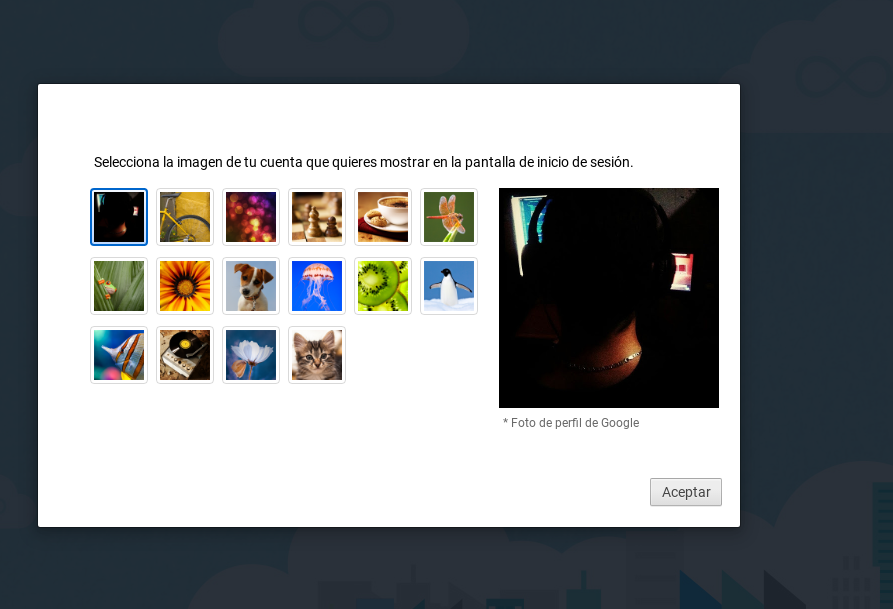
\includegraphics[width=0.68\textwidth]{imgs/6.png}
        }}
	\subfloat[Install wizard terminado, listo para su uso.]{\label{fig:particiones}{
   		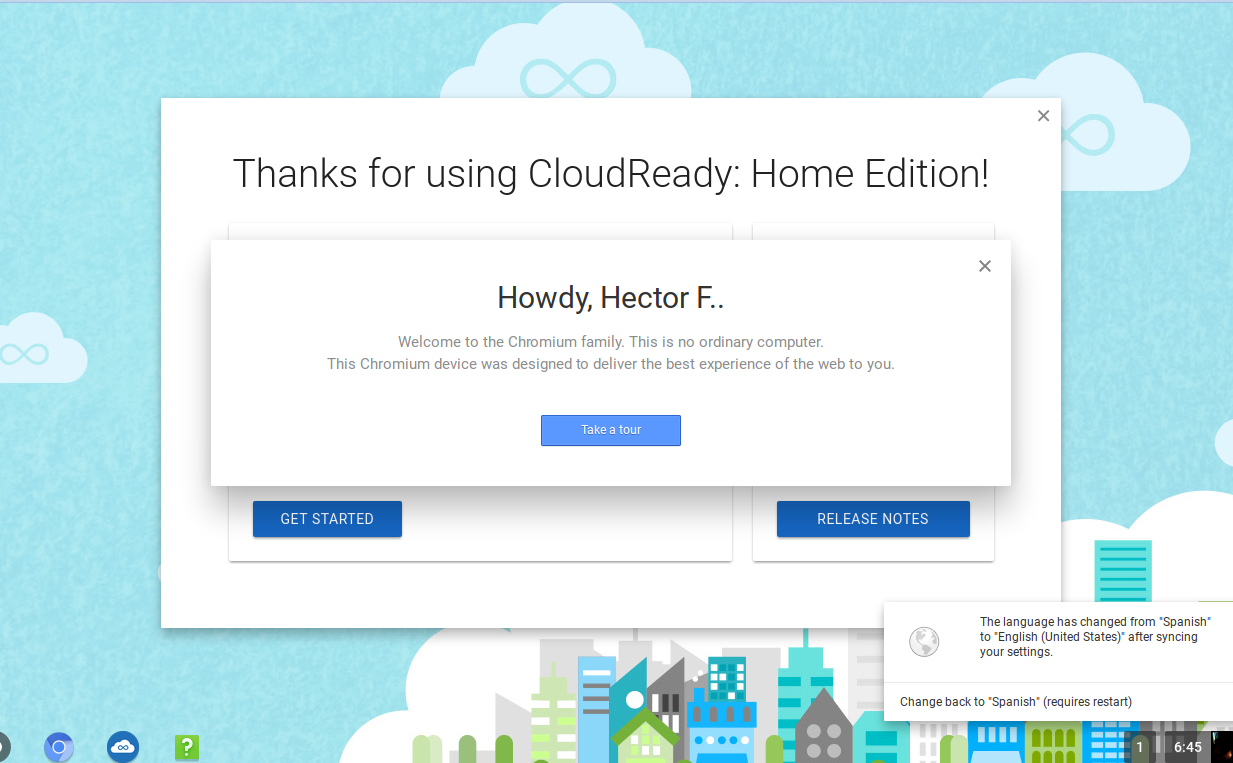
\includegraphics[width=0.68\textwidth]{imgs/7.png}
        }}
	\caption{Configuración inicial de instalación}
\end{figure}
\begin{figure}[H]
 	\centering
   	\subfloat[CloudReady nos da la bienvenida]{\label{fig:bienvenida}{
   		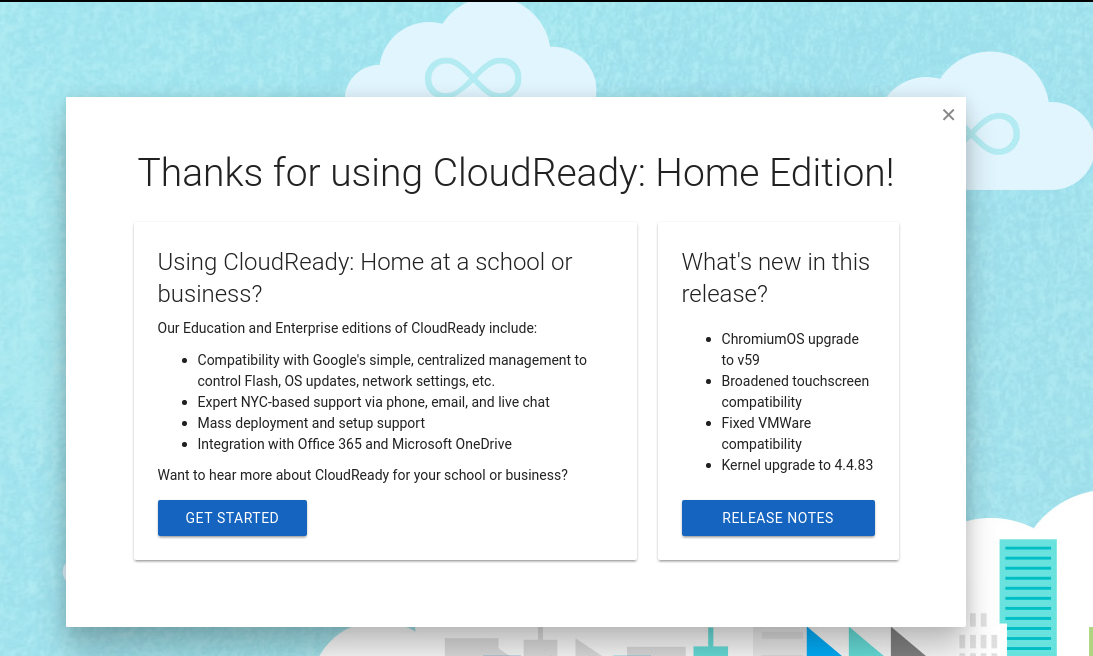
\includegraphics[width=0.68\textwidth]{imgs/8.png}
   		}}
	\subfloat[Prueba de Acceso a terminal Bastante limitada. NO tiene muchos binarios Linux, ni herramientas]{\label{fig:formateada}{
   		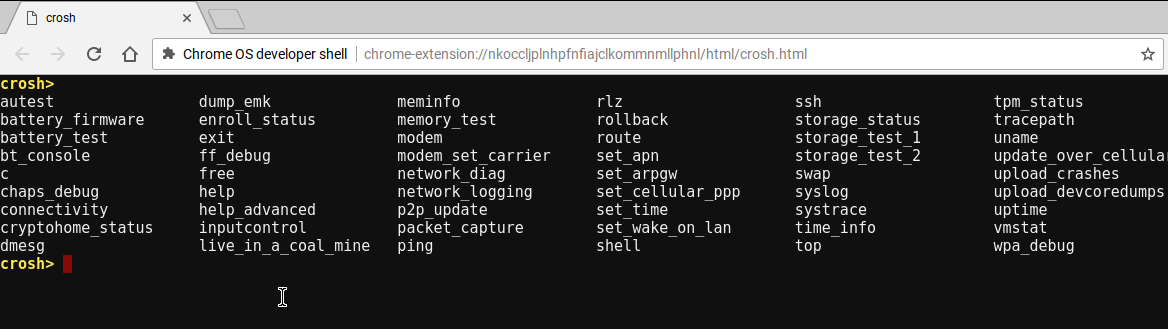
\includegraphics[width=0.68\textwidth]{imgs/9.png}
        }}
       \hfill
	\subfloat[Unicas opciones sistema operativo]{\label{fig:disco}{
   		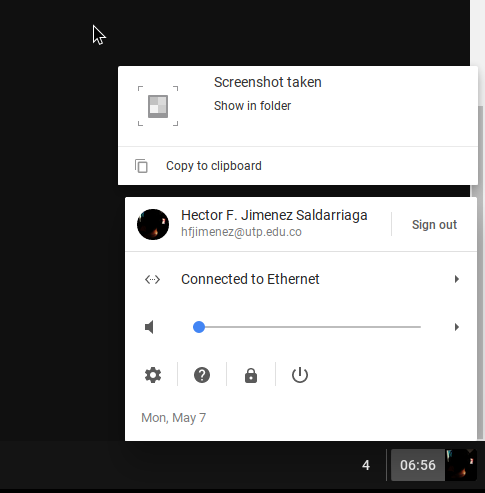
\includegraphics[width=0.68\textwidth]{imgs/10.png}
        }}
      \subfloat[Gestion de Archivos, con mismo navegador.]{\label{fig:ufs}{
   		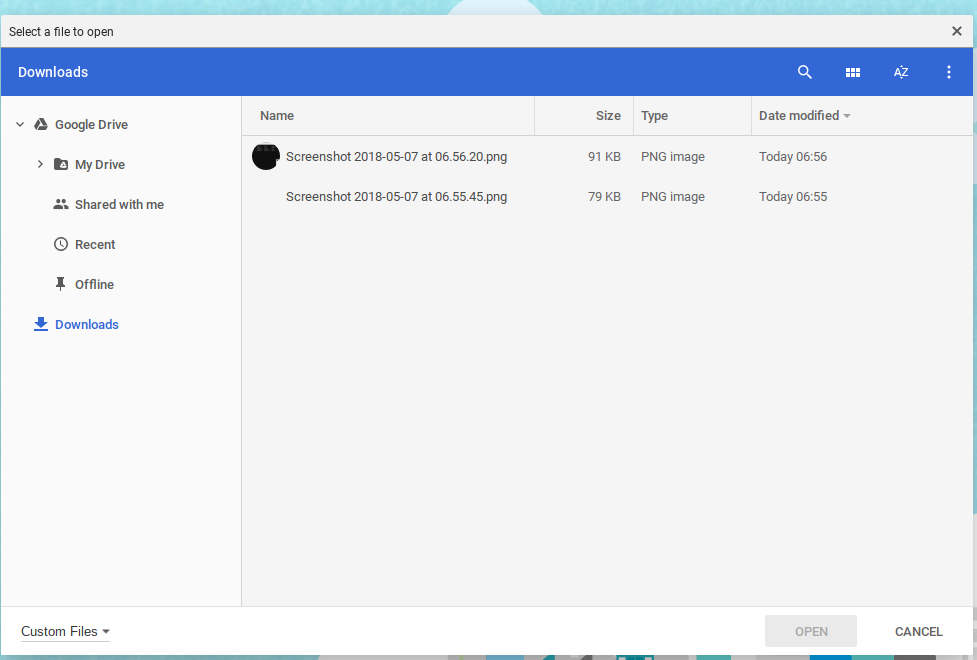
\includegraphics[width=0.68\textwidth]{imgs/11.png}
        }}
	\caption{Proceso secuencial de instalación, Install Wizard Chrome}
\end{figure}
\section{Manejo de Archivos}
\begin{center}
\begin{figure}[H]
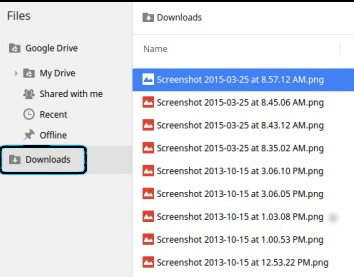
\includegraphics[scale=0.4]{imgs/files.png}
\caption{Chrome OS, Archivos gestion atravez de una aplicación}
\label{fig:files}
\end{figure}
\end{center}
La gestion de archivos dentro del sistema operativo debe se realizado utilizando un software o aplicacion disponible en la chromewebstore. Para ello esto nos permitira : 
\begin{itemize}
\item  Buscar archivos o carpetas
\item  Gestionar todas las operaciones CRUD sobre archivos, carpetas
\item  Renombrar archivos y carpetas
\item  Copiar de archivos o carpetas en ubicaciones diferentes
\end{itemize}

\section{Clasificacion}
Este sistema operativo se clasifica como :
\begin{enumerate}
\item Multiusuario:  Permite multiples inicios de session en la misma maquina, utiliza google service auth para la gestion e inicio de sessiones. 
\item Multitareas: Es posible realizar multiples actividades en la misma maquina al tiempo.
\item Propósito especifico
\item máquina virtual.
\item abierto. 
\end{enumerate}

\end{document}